\documentclass[11pt,a4paper,english]{article}
\usepackage[english]{babel}
\usepackage{marginnote}
\usepackage[utf8]{inputenc}
\usepackage[top=1in]{geometry}

\usepackage{graphicx} %behandle grafikk
\usepackage{float}
\usepackage[hidelinks]{hyperref} %trykkbar referering
\usepackage{gensymb}

\newenvironment{loggentry}[2]% date, heading
{\noindent\textbf{#2}\marginnote{#1}\\}{\vspace{0.5cm}}


\title{UNIK4690 Project}
\author{
  Akhsarbek Gozoev  - akhsarbg \\
  Sadegh Hoseinpoor - sadeghh\\
  Key Long Wong - keylw
}


\begin{document}

\maketitle
\section*{Project description}
\textbf{The purpose of the software is to recognise text from any
surface with uneven lighting. Hence this falls under the ``Optical character recognition'' (OCR) problem}

\noindent \\ As OCRs are still a challenging task even for companiese like
Google, ref. reader to Googles OCR translator application on smartphones,
drawbacks such as; difficulty finding all the text on the photo becasue of
lighting, noise etc., therefore we will have to limit our software significantly.

\noindent \\ \textbf{Initial limitations}
\begin{itemize}
 \item{English alphabet + numbers [0-9]}
 \item{Homogeneous background}
 \item{Computer printed text}
 \item{}
\end{itemize}

\noindent \\ \textbf{Project components}.
\noindent \\ The group have come to the conclusion that the OCR software has
3 main components to it.
\begin{enumerate}
 \item{\textit{Finding text on a photo and returning the text within a bounding box}}
 \item{\textit{Do preprocessing on the segmented text; rotation, greylevel normalization, symbol segmentation}}
 \item{\textit{Classification of the symbols}}
\end{enumerate}
\noindent \\ Additionally there is one more very important component for this
OCR software to work, \textit{\textbf{labled data}}. Even though one might not
need to code for this part, a good poolof labeld data is needed to be able to
classify symbols. More on this under description for this part.
\noindent \\ (4. \textit{Gathering labeled data to train a classification algorithm})
\\

\noindent \\ \textbf{Project INIT}.
\noindent \\ As we want to test the prof of concept first we simplyfied the SW
to just be:
\noindent \\ \textit{\textbf{Recognise numbers [0-9] from a binary img,
with computer printed numbers on homogenous background. Contaioning one
horizontal line of numbers}}
\noindent \\
\noindent \\ \textbf{Second step}
\noindent \\ Assume sequence(n number of lines) of numbers. not horizontal
lines. on homogeneous background.




\newpage
\section*{Report}
\begin{loggentry}{19.04.18}{Week 1}
\begin{itemize}
  \item{Feedback on project proposal}
  \item{Overview of project}
    \begin{itemize}
     \item{simplification}
     \item{binary image $\rightarrow$ numbers $\rightarrow$ straight text $\rightarrow$ Classify}
   \end{itemize}
  \item{init; github - atom}
  \item{first test of charcter Segmentation}
\end{itemize}
\end{loggentry}


\newpage
\begin{loggentry}{26.04.18}{Week 2}
\begin{itemize}
  \item{Charcter Segmentation - Projection Histograms - OpenCV}
  \begin{itemize}
    \item{By projection the histogram of the binary image on the Y-axis,
    we can find where the sentences/lines of text appears. Following, a
    projection histogram on the X-axis can discover where the charecters
    appear.}
  \end{itemize}

  \begin{figure}[H]
    \centering
    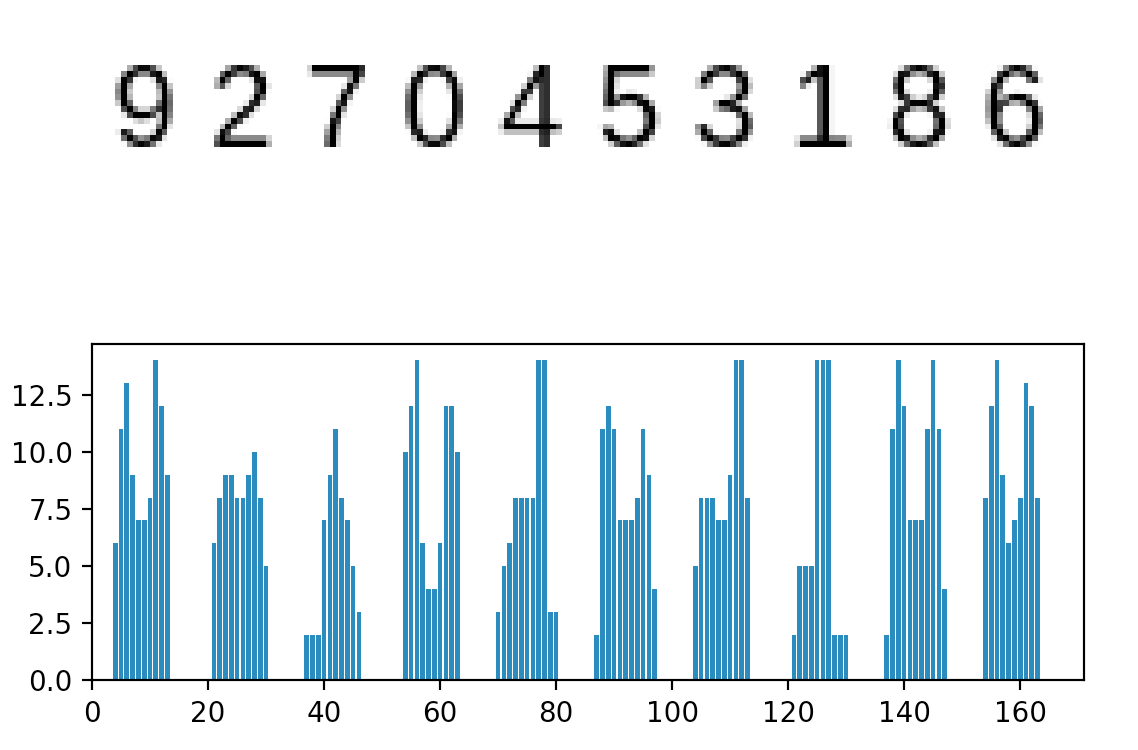
\includegraphics[height=4cm]{res/0-9_segmented_out.png}
    \caption{[0-9] segmented with projection histogram}
    \label{fig:0-9_segmented_out}
  \end{figure}

  \item{Classification - Perceptron neural network - TensorFlow}
    \begin{itemize}
      \item{MNIST dataset - Datasett consisting of several thousand handwritten
      labeled numbers}
      \begin{itemize}
        \item{Numbers ranging from [0-9]}
        \item{Images are 28x28pixels}
      \end{itemize}
      \item{Hyperparameter tuneing}
      \begin{itemize}
        \item{Activation function}
        \item{Number of hidden layers}
        \item{Nodes in hidden layers}
        \item{Cost function}
        \item{Optimazation function}
        \item{Learning rate}
      \end{itemize}
      \item{Theoretic accuracy of the network with 2 hidden layers ~98\%}
      \begin{itemize}
        \item{Measured accuracy ~97\%}

        \begin{figure}[H]
          \centering
          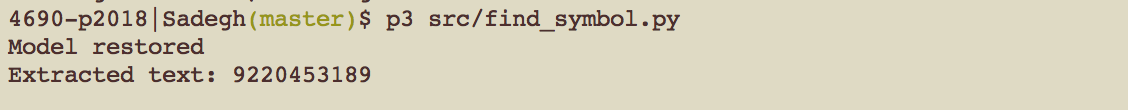
\includegraphics[height=1cm]{res/classification_first_print.png}
          \caption{First output with classification. input see Figure ~\ref{fig:0-9_segmented_out}}
          \label{fig:classification_first_print}
        \end{figure}

      \end{itemize}
    \end{itemize}
\end{itemize}
\end{loggentry}


\newpage
\begin{loggentry}{03.05.18}{Week 3}
\begin{itemize}
  \item{Rotation of text}
  \begin{itemize}
    \item{Hough transform}
    \item{\textit{cv2.minAreaRect()}}
  \end{itemize}
  \item{How to distinguish between upside-down, and verticle vs horisontal text segments}
  \begin{itemize}
    \item{Classifiy in all 4 rotations, and choose the classification with highest avrage confidence}
  \end{itemize}
  \item{Classification - Perceptron neural network - Error}
  \begin{itemize}
    \item{Error rate too high, test-set accuracy 97\%, validation set accuracy $<$ 50\%}
    \item{CNN - TensorFlow Estimator API}
    \begin{itemize}
      \item{Challenging documantation; load/save models}
    \end{itemize}
    \item{Dataset - FNIST - Group contribution}
    \begin{itemize}
      \item{Dataset including several fonts}
      \item{English alphabet, and numbers [0-9]}
    \end{itemize}
  \end{itemize}
\end{itemize}
\end{loggentry}

\newpage
\begin{loggentry}{17.05.18}{Week 4}
\begin{itemize}
  \item{-----}
  \begin{itemize}
    \item{-----}
    \item{-----}
  \end{itemize}
  \item{------}
\end{itemize}
\end{loggentry}

\end{document}
